\documentclass[letterpaper,12pt, oneside, onecolumn, openany]{book}
\usepackage[utf8]{inputenc}
\usepackage{graphicx}
\usepackage[spanish]{babel}
\usepackage[margin=2cm]{geometry}
\usepackage{hyperref}

\begin{document}
	
\title{Proyecto de Desarrollo: Cine+}
\author{Ejecutores:\\
	Carlos Toledo Silva C-311 (l\'ider)\\
	Ayl\'in \'Alvarez Santos C-312\\
	Rocio Ortiz Gancedo C-311\\
	Ariel A. Triana P\'erez C-311}
\date{}
\maketitle
	
\chapter{Introducción}

\section{Prop\'osito del documento}

N/A

\section{Alcance del producto}

N/A

\section{Definiciones, acr\'onimos y abreviaturas}

.NET 5: plataforma que emplea librerías de clase de base unificadas para todos los modelos de apps.

C\#: lenguaje de programación multiparadigma desarrollado y estandarizado por la empresa Microsoft como parte de la plataforma .NET. 

Javascript (JS): es un lenguaje de programación interpretado, se define como orientado a objetos, basado en prototipos, imperativo, débilmente tipado y dinámico.

Hosting: es el servicio que provee a los usuarios de Internet un sistema para poder almacenar información, imágenes, vídeo, o cualquier contenido accesible vía web.

Dominio: nombre único que identifica una subárea de Internet.
Posicionamiento Search Engine Optimization: (posicionamiento SEO) es un conjunto de acciones orientada a mejorar el posicionamiento de un sitio web en la lista de resultados de Google, Bing, u otros buscadores de internet. El SEO trabaja aspectos técnicos como la optimización de la estructura y los metadatos de una web, pero también se aplica a nivel de contenidos, con el objetivo de volverlos más útiles y relevantes para los usuarios.

SQLite: es un Sistema de gestión de bases de datos relacional.

HTTP: protocolo orientado a transacciones y sigue el esquema petición-respuesta entre un cliente y un servidor. Su siglas vienen de Hypertext Transfer Protocol

HTTPS: es un protocolo de aplicación basado en el protocolo HTTP, destinado a la transferencia segura de datos de hipertexto.
Certificado SSL: protocolos criptográficos, que proporcionan comunicaciones seguras en una red.

\section{Referencias}

\begin{enumerate}
	\item Adam Freeman. Pro ASP.NET Core 3.
	\item Jeffrey Palermo. The Onion Architecture. \href{https://jeffreypalermo.com/2008/07/the-onion-architecture-part-1/amp/}{https://jeffreypalermo.com/2008/07/the-onion-architecture-part-1/amp/} 
\end{enumerate}

\section{Resumen del resto del documento}

N/A

\chapter{Descripción general}

\section{Perspectiva del producto}

El producto busca controlar la venta de entradas de un cine denominado Cine+. Para esto el producto debe dar soporte tanto a la venta de entradas por taquillas como a la venta de entradas por internet, garantizándose la coordinación de las mismas.

\section{Funciones del Producto}

El producto es una aplicación web multiplataforma que permite la compra de entradas a través de su página web por parte de los clientes y calcula el costo de la entradas atendiendo a diferentes parámetros. Además da soporte a la inscripción de usuarios como socios del club de Cine+, así como los beneficios de los que estos pueden disfrutar. También el producto permite la anulación de las compras de entradas por parte de los usuarios y hace las actualizaciones pertinentes dada la anulación. El producto permite además que los gerentes del cine puedan actualizar el listado de películas y horarios disponibles y que estos sean mostrados en la web. Además estos pueden consultar las estadísticas de venta de entradas por diferentes parámetros. También se posibilita la visualización en una página web de las 10 películas sugeridas por uno de los gerentes del cine.

\section{Características de los usuarios}

Con el producto interactuarán tres tipos de usuarios: clientes, taquilleros y gerentes. Los gerentes dominan toda la información relacionada con la puesta en escena de las peliculas: horarios, precios, películas que se mostrarán, sugerencias, etc. Los taquilleros dominan como controlar el sistema de tal forma que la venta de entrada puedea mantenerse coordinada entre la venta física en la taquilla y la venta web. Los 3 tipos de usuarios están identificados tanto con dispositivos móviles y tabletas como con computadoras.

Los gerentes y taquilleros tienen el conocimiento necesario para operar este tipo de aplicación web realizando sus respectivas funciones. Los clientes conforman un grupo muy heterogéneo, algunos no tienen conocimiento con productos similares, ahí la necesidad de que la interfaz con la que interactúan sea cómoda.

\section{Restricciones Generales}

El cliente solicita que el sistema en cuestión sea una aplicación web, con las funcionalidades anteriormente mencionadas. Además informa que ya reservaron el hosting y dominio (www.cine+.com) de la página y la base de datos. El hosting tiene 4000 MB de almacenamiento.

El cliente pide que las páginas carguen en el tiempo recomendado por los expertos en posicionamiento SEO, para el posicionamiento en buscadores como Google o Bing. Además que el sitio tenga un flujo de navegación sencillo, y que la navegación no sobrepase el tercer nivel.

\section{Dependencias y suposiciones}

La aplicación web se desarrollará sobre .NET 5, y C\#, para el manejo de la base de datos se emplea SQLite. Para la optimización del tiempo de respuesta del sitio, se reducirá el tamaño de las imágenes, y la cantidad de script de JS a cargar. 

\chapter{Requerimientos Específicos}\label{ch:req}

\section{Requerimientos funcionales}

El sitio web debe permitir que cualquier usuario pueda comprar entradas. Para ello debe buscar la película deseada y mostrar los horarios y salas en que estará en pantalla dicha película. Luego de que el usuario escoja la sala y el horario de su preferencia, el sistema le pregunta al usuario el número de entradas y asigna unas butacas autómaticamente, pero da opción a que el usuario las modifique a su gusto, las cuales pasarán a estar reservadas de forma provisional. Si pasado algún un tiempo (por defecto 10 min) el usuario no ha efectuado la compra o éste la cancela las butacas vuelven a estar disponibles.

Para el cálculo del precio de la entrada, se deben tener en cuenta los diferentes descuentos que se ofrecen.

Los usuarios que los deseen puden darse de alta como socios del club Cine+, cumpliendo con las pasos pertinentes. A cada socio, cada vez que compre una entrada, se le sumarán 5 puntos, los cuales podrá cambiar en el futuro por entradas. Para hacer esto el socio deberá contar con la suficiente cantidad de puntos para poder pagar todas las entradas de su compra. El precio de la entrada es de 20 puntos por defecto, aunque este se podrá configurar.

La compra por web se realiza por medio de tarjeta de crédito, utilizándose una pasarela de pago segura. En taquilla se admite sólo pago en efectivo. Además se debe poder imprimir un comprobante de venta de las entradas.

Una compra realizada a través de la web puede ser anulada hasta 2 horas antes del comienzo  de la sesión, restableciéndole al cliente el costo de la compra y dejando sus butacas disponibles. Si el pago fue hecho por un socio utilizando sus puntos, estos serán devueltos a su cuenta.

Los gerentes podrán actualizar el listado de películas y los horarios, los cuales serán mostrados en el sittio. Además estos podrán consultar estadísticas sobre las ventas de entradas.

Se exige mostrar una vista de 10 películas sugeridas para ver, la cual será actualizada periódicamente. Estará lista seguirá un criterio escogido por alguno de los gerentes.

\section{Requerimientos no funcionales}

Dado que esta es una aplicación web para la venta de entradas para un cine, se le debe dar bastante información sobre el tema a la aplicación para que un navegador pueda encontrala más rápidamente.

Los datos referentes a las películas (salas, horarios, etc) serán guardados en una base de datos SQLite. En esta se guardará además la información referente a los socios, taquilleros y a los gerentes del cine.

El acceso de los gerentes, los taquilleros y los socios de Cine+ al sistema es a través del nombre de usuario y contraseña. Para el acceso al perfil de usuario es necesario comunicaciones seguras, así como para navegar en la administración para el caso de los gerantes y gestionar las ventas para el caso de los taquilleros. Las mismas también son necesarias para la realización de los pagos mediante la pasarela. Por lo anterior es necesario contratar un certificado SSL para el sitio. En caso de que se acceda a través de HTTP será imposible ingresar  el nombre y la contraseña, así como recuperar contraseñas.

La interfaz del usuario deberá ser tan familiar como sea posible a los usuarios, lo cual dependerá de la experiencia de los mismos en el uso de otras aplicaciones web. Se agregará además una documentación online para los clientes, para los taquilleros y  para los gerentes; donde además la dedicada a los clientes contará con información referente sobre cómo convertirse en un socio de Cine+ y los beneficios que trae serlo.

\section{Requerimientos de Entorno}

Aunque los gerentes y taquilleros del cine pueden poseer una variada gama de dispositivos electrónicos se conece que la administración de Cine+ les proverá de recursos necesarios para la realización de sus funciones. Dicho esto se tiene la seguridad de que cada gerente o taquillero tiene asignado uno de estos dos dispositivos para el acceso:

\begin{enumerate}
	\item Laptop ASUS con procesador Intel Core i7 de 4ta generación con navegador Mozilla Firefox 86.0
	\item Laptop HP con procesador Intel Core i5 de 8va generación con navegador Google Chrome 88.0.4324.104
\end{enumerate}

Además en caso de que el gerente no posea un dispositivo móvil de al menos gama media con el que pueda realizar sus funciones, la administración le proverá de un Samsung Galaxy A10 con conexión a Internet y navegadores como Google Chrome 89.0.4389.72 y Safari 14.0.2. 

Los clientes como se conoce son una masa de usuarios heterogénea, como también lo es la masa de dispositivos que ellos tienen disponibles: laptops, móviles, tabletas todos con distintos tipos de sistemas operativos (Windows, Linux, iOS y Android en distintas versiones). Además, en este grupo de usuarios existen distintos tipos de navegadores como Mozilla Firefox, Google Chrome, Opera, Microsoft Edge, Brave, en distintas versiones de los mismos.

En cuanto al hosting, el cliente tiene disponible uno con Windows Server, con 4000 MB de almacenamiento, 1000 MB de base de datos en SQLite, 1 cuenta de acceso para administración, 1000 conexiones concurrentes, 3 cuentas FTP, 1024 Kbps de velocidad de transferencia, soporte para Javascript, para ASP.NET. La aplicación web se desarrollará sobre .NET 5, y C\#.

Para el servidor se tiene un Intel(R) Core(TM) i7-8250U CPU 2.60 GHz, 2.60 GHz, con 16GB RAM. El servidor con arquitectura física de 64 bit.

\chapter{Anexos}

Para la elaboración del presente se realizaron reuniones del equipo de desarrollo con parte del personal del cliente, los entrevistados fueron:

•	Andy Molina: Gerente principal de Cine+.

•	Juan Acosta: encargado de realizar inscripciones de socios.

•	Rosa Mora: encargada de organizar la cartelera del cine.

Se realizaron 3 reuniones con los entrevistados, 2 con Andy Molina (en un periodo de una semana) y 1 con Juan Acosta y Rosa Mora.

Aqu\'i podemos apreciar una imagen de como se ve la p\'agina principal de la aplicaci\'on.

	\begin{figure}[h]
		\begin{center}
			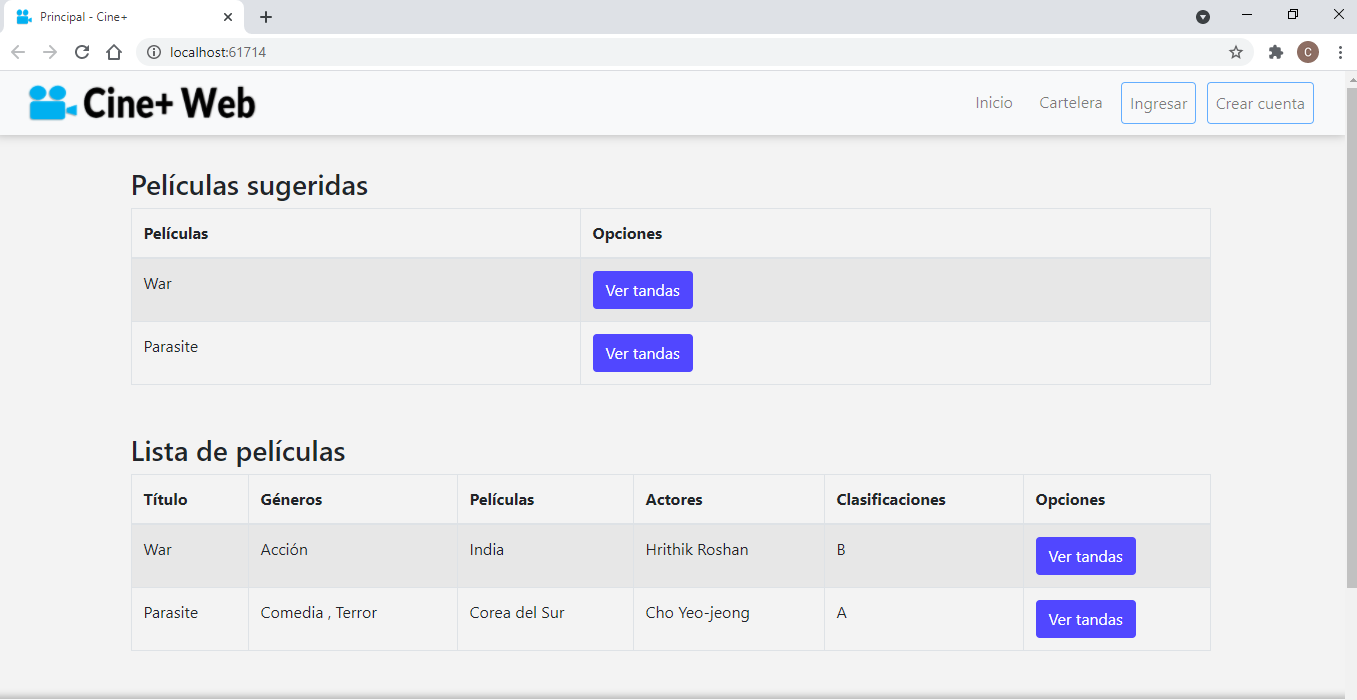
\includegraphics[width =14.0cm]{HomeCine+.png}
		\end{center}
	\end{figure}

\end{document}
